\section{Data Sources}
\label{sec:ui_data_sources}

\begin{figure}[H]
    \hspace*{-2.5cm}
    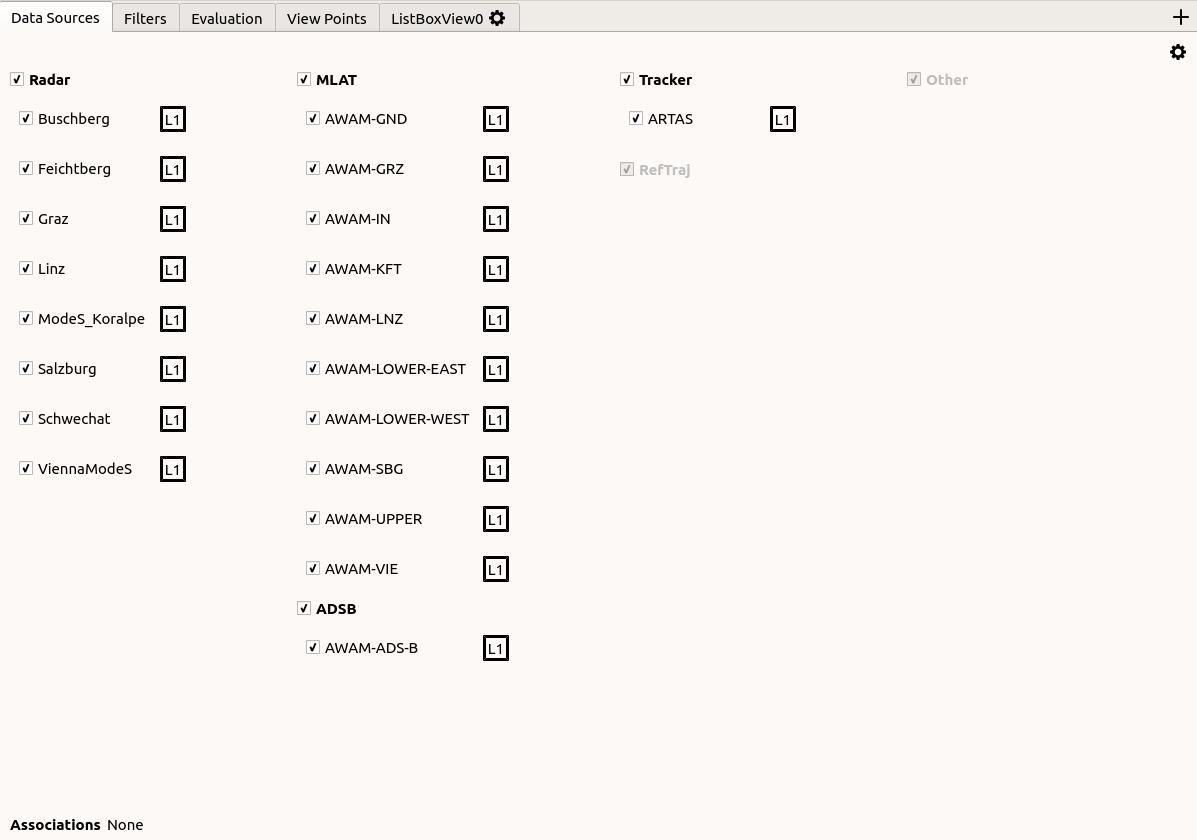
\includegraphics[width=19cm,frame]{figures/ui_data_sources.png}
  \caption{Data Sources Overview}
\end{figure}

In this tab, the data sources existing in the database are shown. Data sources are added to the database if data during the import process was associated to the respective data source (and the respective data source line). \\

Data sources are grouped by DSType (data source type, e.g. Radar, MLAT, ...), and can have up to 4 active lines (L1-L4). Each line for which data exists in the database is shown as a button. \\

Loading of the reppective data can be changed on 3 levels:

\begin{itemize}
 \item By DSType (using checkbox)
 \item By data source (using checkbox)
 \item By data source line (using button, strong border means active)
\end{itemize}
\  \\

At the bottom, the 'Associations' label indicates if association information exists, and from which data source it was generated. 
